\documentclass[10pt,table,mathserif]{beamer}
\usetheme[
%%% options passed to the outer theme
%    hidetitle,           % hide the (short) title in the sidebar
%    hideauthor,          % hide the (short) author in the sidebar
%    hideinstitute,       % hide the (short) institute in the bottom of the sidebar
%    shownavsym,          % show the navigation symbols
%    width=2cm,           % width of the sidebar (default is 2 cm)
%    hideothersubsections,% hide all subsections but the subsections in the current section
%    hideallsubsections,  % hide all subsections
%    right                % right of left position of sidebar (default is right)
  ]{Aalborg}

\setbeamertemplate{theorems}[numbered]

\definecolor{watred}{cmyk}{.00,1,1,0.00}
\definecolor{watyellow}{cmyk}{0,0.12,1,0}
\definecolor{watgray}{cmyk}{0,0,0,0.5}

% If you want to change the colors of the various elements in the theme, edit and uncomment the following lines
% Change the bar and sidebar colors:
\setbeamercolor{Aalborg}{fg=black,bg=watred}
\setbeamercolor{sidebar}{bg=white}
% Change the color of the structural elements:
\setbeamercolor{structure}{fg=red}
% Change the frame title text color:
%\setbeamercolor{frametitle}{fg=blue}
% Change the normal text color background:
\setbeamercolor{normal text}{bg=white, fg=black}
\setbeamercolor{alerted text}{bg=white, fg=red}
% ... and you can of course change a lot more - see the beamer user manual.
\usepackage{xcolor}
\usepackage[utf8]{inputenc}
\usepackage[english]{babel}
\usepackage[T1]{fontenc}
\usepackage{threeparttable}
% ... or whatever. Note that the encoding and the font should match. If T1
% does not look nice, try deleting the line with the fontenc.
\usepackage{lmodern}
\usepackage{subcaption}
\usepackage{algorithm}
\usepackage{algorithmic}
\usepackage{colortbl}
\usepackage{biblatex}
\usepackage{bibentry}
\usepackage{epstopdf}
\usepackage{caption}
\usepackage{multirow}
\usepackage{animate}
\usepackage{tikz}
\usetikzlibrary{shapes}
\usetikzlibrary{arrows}
\usetikzlibrary{positioning, fit, arrows.meta}
\usepackage{tkz-graph}
\usetikzlibrary{backgrounds,automata}
\bibliography{mybib.bib}



\newcommand*{\Scale}[2][4]{\scalebox{#1}{$#2$}}%
\newcommand*{\Resize}[2]{\resizebox{#1}{!}{$#2$}}%
\newcommand{\vt}[1]{\mathbf{#1}}
\newcommand{\vw}{\mathbf{w}}
%\newcommand{\pm}{\stackrel{+}{-}}
\newcommand{\vx}{\mathbf{x}}
\newcommand{\vi}{\mathbf{i}}
\newcommand{\vo}{\mathbf{o}}
\newcommand{\vxt}{\tilde{\mathbf{x}}}
\newcommand{\vy}{\mathbf{y}}
\newcommand{\impsigma}{\breve{\sigma}}
\newcommand{\barK}{\overline{K}}
\newcommand{\barC}{\overline{C}}
\newcommand{\vz}{\mathbf{z}}
\newcommand{\fnp}{\tilde{f}}
\newcommand{\vu}{\mathbf{u}}
\newcommand{\vs}{\mathbf{s}}
\newcommand{\vc}{\mathbf{c}}
\newcommand{\E}{\mathbf{E}}
\newcommand{\HK}{\mathcal{H}_K}
\newcommand{\XS}{\mathcal{X}}
\newcommand{\DS}{\Delta S}
\newcommand{\Heston}{\textsc{Heston}}
\newcommand{\DVmkt}{\Delta \breve{V}}
\newcommand{\DT}{\Delta_t}
\newcommand{\vuu}{\mathbf{\widetilde u}}
\newcommand{\Real}{\mathbb{R}}
\newcommand{\vdot}[2]{{#1}^T{#2}}
\DeclareMathOperator*{\argmin}{\arg\!\min}
\newcommand{\sym}{\textsc{sym}}
\newcommand{\BS}{\textsc{BS}}
\newcommand{\LOF}{\textsc{lof}}
\newcommand{\svm}{\textsc{svm}}
\newcommand{\AMflag}{\text{mFLAG}}
\newcommand{\rw}{\textsc{rw}}
\newcommand{\diag}{\textsc{diag}}
\newcommand{\sign}{\textsc{sign}}
\newcommand{\MeanAbs}{\E(|\DVmkt-\DS f(\vx)|)}
\newcommand{\Cluster}{\textsc{C}}
\newcommand{\bi}{\text{bi}}
\newcommand{\g}{\mathbf{g}}
\newcommand{\vv}{\mathbf{v}}
\newcommand{\valpha}{\pmb{\alpha}}
\newcommand{\vK}{\pmb{K}}
\newcommand{\vV}{\pmb{\breve{V}}}
\newcommand{\e}{\mathbf{e}}
\newcommand{\vol}{\upsilon}
\newcommand{\vd}{\mathbf{d}}
\newcommand{\vh}{\mathbf{h}}
\newcommand{\vf}{\mathbf{f}}
\newcommand{\vW}{\pmb{W}}
\newcommand{\np}{\text{np}}
\newcommand{\pt}{^{+\Delta t}}
\newcommand{\norm}{\text{norm}}
\newcommand{\row}{\text{row}}
\newcommand{\Vmkt}{\breve{V}}
\newcommand{\vecVmkt}{\mathbf{\breve{V}}}
\newcommand{\Ncut}{\text{Ncut}}
\newcommand{\half}{\frac{1}{2}}
\newcommand{\DKLs}{\bf\textsc{DKL}_{\text{SPL}}}
\newcommand{\DKLg}{\bf\textsc{DKL}_{\text{RBF}}}
\newcommand{\IKLs}{\bf\textsc{IKL}_{\text{SPL}}}
\newcommand{\IKLg}{\bf\textsc{IKL}_{\text{RBF}}}
\newcommand{\LVF}{\textsc{LVF}}
\newcommand{\Del}{\delta^{\textsc{BS}}}
\newcommand{\SABR}{\bf\textsc{SABR}}
\newcommand{\MV}{\bf \textsc{MV}}
\newcommand{\vU}{\pmb{U}}
\newcommand{\vb}{\mathbf{b}}




\nobibliography{Ref.bib}
\definecolor{mycyan}{cmyk}{.2,0,0,0}
\definecolor{mycyan1}{cmyk}{.1,0,0,0}
\definecolor{mycyan3}{cmyk}{.3,0,0,0}
% colored hyperlinks
\newcommand{\chref}[2]{%
  \href{#1}{{\usebeamercolor[bg]{Aalborg}#2}}
}

\title[Option Data Augmentation]% optional, use only with long paper titles
{Option Data Augmentation Using SABR model and Local Volatility Function}


\author[Ke Nian ] % optional, use only with lots of authors
{ Ke Nian\\
 Supervisors: Prof.Yuying Li and Prof.Thomas.F.Coleman
}


% - Give the names in the same order as they appear in the paper.
% - Use the \inst{?} command only if the authors have different
%   affiliation. See the beamer manual for an example

%specify some optional logos
\pgfdeclareimage[height=1.4cm]{mainlogo}{logo.png} % placed in the upper left/right corner
\logo{\pgfuseimage{mainlogo}}

\pgfdeclareimage[height=0.75cm]{logo2}{tu-logo} % placed in the lower left/right corner if the \pgfuseimage{logo2} command is uncommented in the \institute command below

\institute[
%  {\pgfuseimage{logo2}}\\ %insert a company or department logo
  David R. Cheriton School of Computer Science, University of Waterloo
] % optional - is placed in the bottom of the sidebar on every slide
{%
  David R. Cheriton School of Computer Science,\\
  University of Waterloo,\\
  Waterloo, Canada
  %there must be an empty line above this line - otherwise some unwanted space is added between the university and the country (I do not know why;( )
}
\date{\today}

\begin{document}
% the titlepage
\begin{frame}[plain] % the plain option removes the sidebar and header from the title page
  \titlepage
\end{frame}
%%%%%%%%%%%%%%%%

% TOC
\begin{frame}{Agenda}{}
\tableofcontents
\end{frame}
%%%%%%%%%%%%%%%%
\section{Introduction}
\subsection{Overview of the Discrete Hedging Problem}
\begin{frame}{Set Up Self-Financing Portfolio}
Consider a portfolio $P_{t}$ which is composed of:
\begin{itemize}
	\item A short position on option $V_t$
	\item Long $\delta_t$ (hedging position) shares of $S_t$
	\item An amount in a risk-free bank account $B_t$
\end{itemize}
The hedging portfolio is rebalanced at discrete times $t_i$. The hedging position is given by $\delta_{t_i}$
Initially, we have
\[
P_{t_0}=  -V_{t_0}+\delta_{t_0} S_{t_0}+ B_{t_0}=0
\]
And
\[
B_{t_0}=V_{t_0}-\delta_{t_0} S_{t_0}
\]
\end{frame}

\begin{frame}{Rebalance Self-Financing Portfolio}
At each rebalancing time $t_i$, we update our hedging position by change the share we hold from $\delta_{t_{i-1}}$ to $\delta_{t_i}$ at $t_i$, where any required cash is borrowed, and any excess cash is loaned. Assume $\Delta t=t_{i}-t_{i-1}$ is fixed.
The bank account is updated by:
\[
B_{t_{i}}=e^{r \Delta t} B_{t_{i-1}}-S_{t_i}(\delta_{t_i}-\delta_{t_{i-1}})
\]
\end{frame}


\begin{frame}{Hedging Objective}
Let $t_i^+$ and $t_i^-$  to be the time immediately after  and immediately before $t_i$. Assume that the performance is measured at the $t_N$:
\[ \begin{split}
P_{t_N^-}&=e^{r \Delta t} B_{t_{N-1}}- V_{t_N}+ S_{t_N} \delta_{t_{N-1}}  \\
&=\sum_{j=0}^{N-1}\left\{ \left[e^{r (N-j-1) \Delta t} S_{t_{j+1}}-e^{r (N-j) \Delta t}S_{t_{j}}\right] \delta_{t_i} \right\}\\
&+e^{r N \Delta t} V_{t_0}-V_{t_N}
\end{split}
\]

If we always set $\delta=\frac{\partial V}{\partial S}$ and let $\Delta t \rightarrow 0$ (we continuously rebalance the portfolio), then $P_{t_N^-}=0$. In reality, we can only rebalance discretely and  $P_{t_N^-}$ can take positive (profit) and negative value (loss).
\end{frame}


\begin{frame}{Data-Driven Total Hedging Objective}
Assume we have $M$ samples of sequences. Each sequence is of length N. Let the hedging position given by a function $\delta_t = f (X_t,y_t)$.
The objective of optimizing $f$ is:
\[
\min_{f} \;\;\frac{1}{2 M} \sum_{i=1}^M (P^i_{t_N^-})^2
\]
Where $P^i_{t_N^-}$ is the portfolio at $t_N^-$ of sample $i$:
\[ \begin{split}
P^i_{t_N^-} &=\sum_{j=0}^{N-1}\left\{ \left[e^{r (N-j-1) \Delta t} S^i_{t_{j+1}}-e^{r (N-j) \Delta t}S^i_{t_{j}}\right] f(\mathbf{X}^i_{t_j},\vy^i_{t_{j}})\right\}\\
&+e^{r N \Delta t} V^i_{t_0}-V^i_{t_N}
\end{split}
\]
\end{frame}

\subsection{Challenges of Obtaining Real Data}
\begin{frame}{Challenges of Obtaining Real Data}
The success of building a data-driven model depends on the number of sample paths $M$. However, the hedging sequence we can gather from real market is limited.
\begin{enumerate}
	\item Options with specific K and expiry are not traded every day.
	\begin{itemize}
		\item Interpolation and extrapolation for strikes using SABR Model
	\end{itemize}
	\item Options in real market only have fixed expiry dates:
		\begin{itemize}
		\item Interpolation for expiries using LVF
	    \end{itemize}
\end{enumerate}
\end{frame}


\begin{frame}{Arbitrage-Free Surface}
Simple interpolation (e.g cubic spline) for strikes and expiries can be problematic:
\begin{enumerate}
	\item Simple interpolation can create arbitrage.
	\item Extrapolation is needed for deep in-money option and deep out-of-money option.
	
\end{enumerate}
We want to create a price surface that is \textbf{arbitrage-free}. In addition, we want to \textbf{extrapolate} for deep in-money options and deep out-of-money options.
\end{frame}


\begin{frame}{Static Arbitrage}
Let  $C(T,K)$ be the continuous call price surface function.
\begin{enumerate}
		\item No call spread arbitrage:
		\[
		-1 \leq \frac{\partial C(T,K)}{ \partial K} \leq 0
		\]
		\item  No butterfly spread arbitrage:
		\[
		\frac{\partial^2 C(T,K)}{ \partial K^2} \geq 0
		\]
		\item  No calendar spread arbitrage:
		\[
		\frac{\partial C(T,K)}{ \partial T} \geq 0
		\]
\end{enumerate}
\end{frame}


\section{SABR Model}
\subsection{Model Specification and Calibration}

\begin{frame}{SABR Model}
In the SABR (Stochastic Alpha, Beta, Rho)  model, the asset forward $F$ follows the following stochastic differential equation:
\[
\begin{split}
dF_t&=\sigma_t (F_t)^{\beta}dW_t\\
d\sigma_t&=\alpha \sigma_t( \rho dW_t+\sqrt{1-\rho^2} dZ_t)\\
&dW_t, dZ_t \; \text{\; are\; independent}
\end{split}
\]
where $F_t=F(t,T)=S_te^{(r-q)(T-t)}$ with $r$ be the interest rate and $q$ be the dividend yield.  The constant parameters $\beta ,\alpha$  satisfy the conditions $0\leq \beta \leq 1,\alpha \geq 0$, $\alpha$  is a volatility-like parameter for the volatility. $ \rho$  is the instantaneous correlation between the underlying and its volatility.
\end{frame}

\begin{frame}{Black Model and Implied Volatility}
The price of a European call option on $F$ with exercise date
$T$
\[
C = D(t,T){\mathbb E}[(F_{T}-K)^+]
\]
where ${\mathbb E}[\cdot]$ is under the risk-neutral measure. $D(t,T)=e^{-r(T-t)}$. Market convention often
quotes the price through Black's formula, with $\tau=T-t$
\[
C_B =  D(t,T)[F_tN(d_+)-KN(d_-)], \; d_{\pm} =
\frac{\log(F_t/K)\pm \frac{1}{2}\sigma_B^2
	\tau}{\sigma_B\sqrt{\tau}}.
\]

The remaining problem is how to obtain the implied volatility $\sigma_B=\sigma_B(K,F,\tau)$.
\end{frame}



\begin{frame}{Implied Volatility Approximation Under SABR model}
\[	\tiny
\begin{split}
\sigma_B(K,F,\tau) &\approx
\frac{\sigma_0}{(FK)^{(1-\beta)/2}\left[1+\frac{(1-\beta)^2}{24}\log^2(F/K)
	+ \frac{(1-\beta)^4}{1920}\log^4(F/K) + \cdots\right]} \cdot
\frac{z}{x(z)}  \\
&  \cdot \left\{1+\left[\frac{(1-\beta)^2}{24}\frac{\sigma_0^2}{(FK)^{1-\beta}}
+ \frac{1}{4} \frac{\rho\beta\sigma_0\alpha}{(FK)^{(1-\beta)/2}} +
\frac{2-3\rho^2}{24}\alpha^2 \right]\tau+\cdots\right\}
\end{split}
\]
where $\sigma_0$ is the initial volatility
\[\tiny
z = \frac{\alpha}{\sigma_0}(FK)^{(1-\beta)/2}\log (F/K)\]
\[ x(z) =
\log\left\{\frac{\sqrt{1-2\rho z + z^2}+z-\rho}{1-\rho}\right\}
\]

\end{frame}



\begin{frame}{Model Calibration}
The model calibration of SABR is to match implied volatility approximation $\sigma_B(K,F_t,\tau)$ from SABR model to the market observed $\sigma^{MKT}_B(K,F_t,\tau)$. This can be done by solving a optimization problem with the parameters to be $\alpha,\rho,\sigma_0$. $\beta$ is usually predetermined and not optimized together with other parameters.
\end{frame}


\begin{frame}{Benefit of The SABR model}
The benefits of SABR model are:
\begin{enumerate}
	\item  Matching the volatility smile very well.
	\item  Extrapolation to in-money and  out-of-money options.
	\item  Pricing vanilla options is straightforward.
	\item  Accurate and efficient implied volatility computation.
\end{enumerate}
\end{frame}
\subsection{Interpolation and Extrapolation for Strikes using SABR Model}
\begin{frame}{Interpolation and Extrapolation for Strikes}
The process of interpolation and extrapolation for strikes using SABR Model is
\begin{enumerate}
	\item  Fit $\sigma_B(K,F_t,\tau)$ to the market implied volatility smile for each expiry $T$.
	\item  Compute the European call or put price by plugging in the $\sigma_B(K,F_t,\tau)$ for any K into the black pricing formula.
	\[
	C_{SABR}(T,K) =  D(t,T)[F_t N(d_+)-KN(d_-)]\]
	
	 \[d_{\pm} =
	\frac{\log(F_t/K)\pm \frac{1}{2}\sigma_B^2(K,F_t,T-t)
		\tau}{\sigma_B(K,F_t,T-t)\sqrt{T-t}}
	\]
\end{enumerate}
\end{frame}



\section{Local Volatility Function (LVF)}
\subsection{Dupire's Equation}
\begin{frame}{Dupire's Equation}
The Dupire formula enables us to deduce the volatility function in a local volatility
model from quoted put and call options in the market.
\begin{itemize}
	\item Under a risk-neutral measure, we assume:
	\[
	\frac{d S_t}{ S_t}= \left(r-q\right)dt +\sigma(t,S_t) dZ_t
	\]
	\item Let C be the call option pricing function. Dupire's equation states:
	\[
	\frac{\partial C}{\partial T}=\frac{1}{2} {\sigma}^2(T,K)K^2  \frac{\partial^2 C}{ \partial K^2}-(r-q) K\frac{\partial C}{\partial K}-qC
	\]
\end{itemize}
\end{frame}

\begin{frame}{Dupire's Equation Using Forward Price}
Define the normalized call price in terms of discount factor $D(t,T)$ and forward price $F(t,T)$ and the moneyness $\kappa$ as:
\[
\begin{split}
D(t,T)&=e^{-r(T-t)}\\
F(t,T)&=S_te^{(r-q)(T-t)}\\
\kappa&=\frac{K}{F(t,T)}\\
\widehat{C}(T,\kappa)&=\frac{C(T,\kappa F(t,T))}{D(t,T)F(t,T)}=\frac{C(T,K)}{D(t,T)F(t,T)}
\end{split}
\]
Dupire's equation can be rewritten as:
\[
\frac{\partial \widehat{C}}{\partial T}=\frac{1}{2} \widehat{\sigma}^2(T,\kappa) \kappa^2  \frac{\partial^2 \widehat{C}}{ \partial \kappa^2},\;\; \widehat{\sigma}(T,\kappa)={\sigma}(T,K)
\]
\end{frame}

\subsection{Interpolation  for Expiries using LVF}

\begin{frame}{Interpolation  for Expiries using LVF}
The purpose of volatility Interpolation \footnotemark \; is to create a price surface that can be used to obtain option price with unobserved expiries from market. We recursively solve the finite difference  discretization of the Dupure forward equation using fully implicit method:
\[
\frac{\partial \widehat{C}}{\partial T}=\frac{1}{2} \widehat{\sigma}^2(T,\kappa) \kappa^2  \frac{\partial^2 \widehat{C}}{ \partial \kappa^2}
\]
with initial condition $\widehat{C}(0,\kappa)=max(1-\kappa,0)$, lower boundary condition $\widehat{C}(T,0)=1$, upper boundary condition $\widehat{C}(T,\kappa_{max})=0$
\footnotetext[1]{Jesper Andreasen and Brian Huge. "Volatility interpolation." Risk, 24(3):76, 2011.}
\end{frame}

\begin{frame}{Volatility Interpolation and Option pricing}
Given a grid of expiries $0=T_0 < T_1 < \dots< T_{max} $ and  the grid of moneyness: $0=\kappa_0<\kappa_1<\dots<\kappa_{max}$ and a expiry $T_i$ , we assume $\sigma(T_i,K)$  to be a piecewise constant functions for a given $T_i$. We further assume:
\[
 \frac{\partial^2 \widehat{C}(T,0)}{ \partial \kappa^2}=\frac{\partial^2 \widehat{C}(T,\kappa_{max})}{ \partial \kappa^2}=0
\]
\end{frame}


\begin{frame}{Volatility Interpolation Matrix Form}

The fully implicit finite difference method in matrix form is, where $M$ is a tri-diagonal matrix parametrized by  $\sigma(T_i,.)$:

\[\begin{bmatrix}
\widehat{C}(T_{i},\kappa_0)\\
\widehat{C}(T_{i},\kappa_1)\\
\widehat{C}(T_{i},\kappa_2)\\
\vdots\\
\widehat{C}(T_{i},\kappa_{max})
\end{bmatrix}=M
\begin{bmatrix}
\widehat{C}(T_{i+1},\kappa_0)\\
\widehat{C}(T_{i+1},\kappa_1)\\
\widehat{C}(T_{i+1},\kappa_2)\\
\vdots\\
\widehat{C}(T_{i+1},\kappa_{max})
\end{bmatrix}
\]

\end{frame}


\begin{frame}{Model Calibration}
\[M^{-1} \begin{bmatrix}
\widehat{C}(T_{i},\kappa_0)\\
\widehat{C}(T_{i},\kappa_1)\\
\widehat{C}(T_{i},\kappa_2)\\
\vdots\\
\widehat{C}(T_{i},\kappa_{max})
\end{bmatrix}=
\begin{bmatrix}
\widehat{C}(T_{i+1},\kappa_0)\\
\widehat{C}(T_{i+1},\kappa_1)\\
\widehat{C}(T_{i+1},\kappa_2)\\
\vdots\\
\widehat{C}(T_{i+1},\kappa_{max})
\end{bmatrix}
\]
We try to find M that so that $\widehat{C}(T_{i+1},\kappa_j)=\widehat{C}_{SABR}(T_{i+1},\kappa_j)$.
\[
\widehat{C}_{SABR}(T_{i+1},\kappa_j)=\frac{C_{SABR}(T,K_j)}{D(t,T_{i+1})F(t,T_{i+1})}
\]
\[
K_j=\kappa_j F(t,T_{i+1})
\]
This can be done by:
\[
\inf_{\sigma(T_i,.)} \sum_{j}(\frac{\widehat{C}(T_{i+1},\kappa_j)-\widehat{C}_{SABR}(T_{i+1},k_j)}{Vega_{B}(T_{i+1},\kappa_j)})^2
\]
\end{frame}


\begin{frame}{Interpolation For Expiries}
After optimization,  the local volatility functions are translated into arbitrage-consistent prices for a discrete set of expiries but it does not directly specify the option prices between the expiries.  For $T \in [T_i,T_{i+1})$, we can fill in the gaps by:
\[
\frac{\widehat{C}(T,\kappa) -\widehat{C}(T_{i},\kappa)}{T-T_{i}}=\frac{1}{2}\widehat{\sigma}^2(T_i,\kappa) \kappa^2 \frac{\partial^2 \widehat{C}(T,\kappa) }  {\partial \kappa^2}
\]
We then recover the call price by:
\[
C(T,K)=\widehat{C}(T,\kappa){D(t,T)F(t,T)}
\]
\end{frame}


\begin{frame}{Benefits of Interpolation Based On Local Vol Model}
Interpolation based on the above procedure can guarantee the option price given by interpolation is arbitrage-free:
\begin{enumerate}
	\item No call spread arbitrage:
	\[
	-1 \leq \frac{\partial C(T,K)}{ \partial K} \leq 0
	\]
	\item  No butterfly spread arbitrage:
	\[
	\frac{\partial^2 C(T,K)}{ \partial K^2} \geq 0
	\]
	\item  No calendar spread arbitrage:
	\[
	\frac{\partial C(T,K)}{ \partial T} \geq 0
	\]
\end{enumerate}
\end{frame}

\section{Arbitrage-Free Condition}
\begin{frame}{Arbitrage in SABR Model}
\begin{itemize}
	\item Although SABR model is convenient, it is not arbitrage-free. Butterfly and call spread arbitrage can exist for low strike.
	\item For each expiry, a separate set SABR parameters are calibrated so calender spread arbitrage can also exist.
	\item Therefore, before using the SABR price as the target for the LVF calibration, we need to fix the potential arbitrage.
\end{itemize}
\end{frame}

\begin{frame}{Check for Arbitrage}
 Given the grid of strikes: $0=K_0<K_1<\dots<K_{max}$, and a grid of expiries $0=T_0 < T_1 < \dots< T_{max} $, let $C_{i,j}=C_{SABR}(T_i,K_{j})$, we can check and fix
\begin{itemize}
	\item No call spread arbitrage:
	\[
	0 \leq \frac{C_{i,j-1}-C_{i,j-1}}{K_j-K_{j-1}} \leq 1
    \]
    \item No butterfly spread arbitrage:
    \[C_{i,j-1}-
    \frac{K_{j+1}-K_{j-1}}{K_{j+1}-K_{j}}C_{i,j}+\frac{K_{j}-K_{j-1}}{K_{j+1}-K_{j}C_{i,j+1}} \geq 0
    \]
    \item No calender spread arbitrage:
    \[C_{i+1,j}-C_{i,j} \geq 0 \]
\end{itemize}
\end{frame}




\section{Calibration for SP500 Index Option}
\begin{frame}{SABR Model Calibration Results}
\begin{figure}
	\animategraphics[loop,controls,width=\linewidth]{200}{Sabr/Sabr}{2}{15}
\caption{The Price Surface and Implied Vol Surface for 2012-01-04 SP500 index option}
\end{figure}
\end{frame}

\begin{frame}{LVF Model Calibration Results}
\begin{figure}
	\begin{subfigure}[b]{0.49\textwidth}
		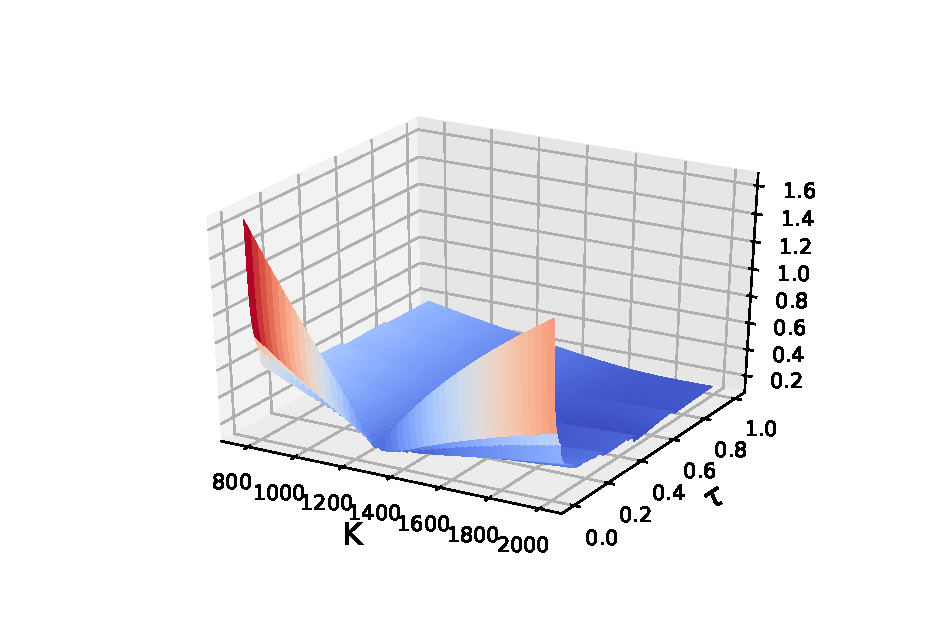
\includegraphics[width=\textwidth]{ImpVol}
		\caption{ImpVol}
	\end{subfigure}
	\begin{subfigure}[b]{0.49\textwidth}
		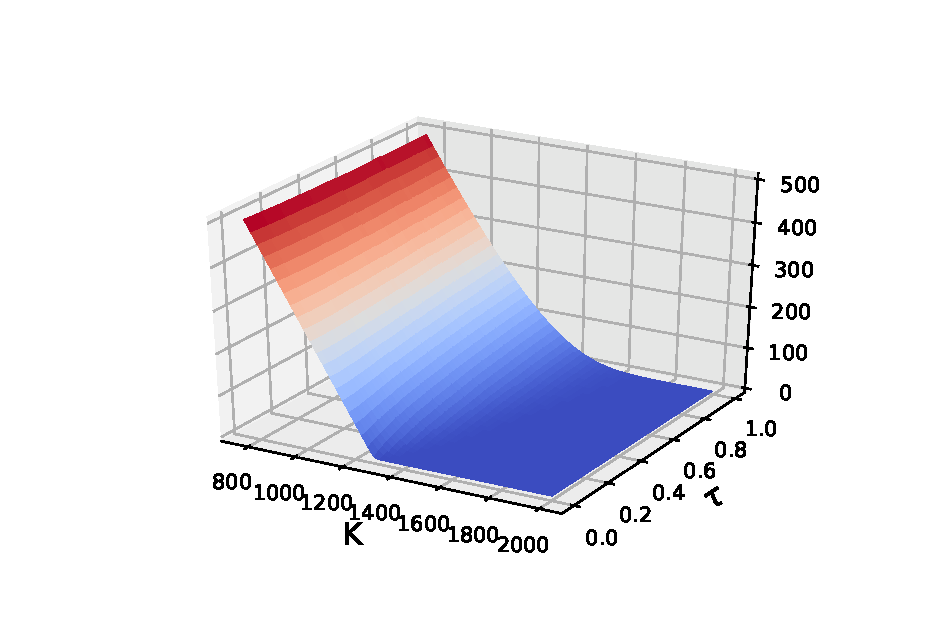
\includegraphics[width=\textwidth]{Price}
		\caption{Price}
	\end{subfigure}
	\caption{The Price Surface and Implied Vol Surface for 2012-01-04 SP500 index option}
\end{figure}
\end{frame}

\section{Hedging in SABR model}
\begin{frame}{Hedging in SABR model}
Based on SARR model, a correction formula for BS delta hedging is given by:
\[
\delta_{SABR}=\frac{\partial C_{B}}{\partial F} + \frac{\partial C_{B}}{\partial \sigma_B}
\frac{\partial \sigma_B}{\partial F}
\]
The first term is the regular Black delta.
The second term is the SABR model's correction to the risk-Black vega times the predicted change in the implied volatility $\sigma_B$ caused by the change in the forward $F$.
\end{frame}


\begin{frame}{Problem with $\delta_{SABR}$ }
Let the SABR implied volatility after calibration be
\[
\sigma_B(K,F,\tau;\alpha,\beta,\rho,\sigma_0)
\]
$\delta_{SABR}$ assume $\sigma_0$  is fixed. However, the $\sigma$ and $F$ are correlated, whenever $F$ changes, $\sigma_0$ changes.
\end{frame}


\begin{frame}{Bartlett Corrective Formula}
Assume:
\[
\begin{split}
dF_t&=\sigma_t (F_t)^{\beta}dW_t\\
d\sigma_t&=\alpha \sigma_t( \rho dW_t+\sqrt{1-\rho^2} dZ_t)\\
&dW_t, dZ_t \; \text{\; are\; independent}
\end{split}
\]
We can easily show that:
\[
d\sigma_t=\frac{\rho \alpha}{(F_t)^\beta}dF_t+\alpha \sigma_t \sqrt{1-\rho^2} dZ_t
\]
Therefore, a better Bartlett formula is given by:
\[
\delta_{Bartlett}=\frac{\partial C_{B}}{\partial F} + \frac{\partial C_{B}}{\partial \sigma_B}
\left( \frac{\partial \sigma_B}{\partial F}+\frac{\partial \sigma_B}{\partial \sigma_0}\frac{\rho \alpha}{ F^{\beta}}\right)
\label{eq:bartlett}
\]
\end{frame}
\begin{frame}{Comparison between $\delta_{SABR}$ and $\delta_{Bartlett}$ }
\begin{figure}
	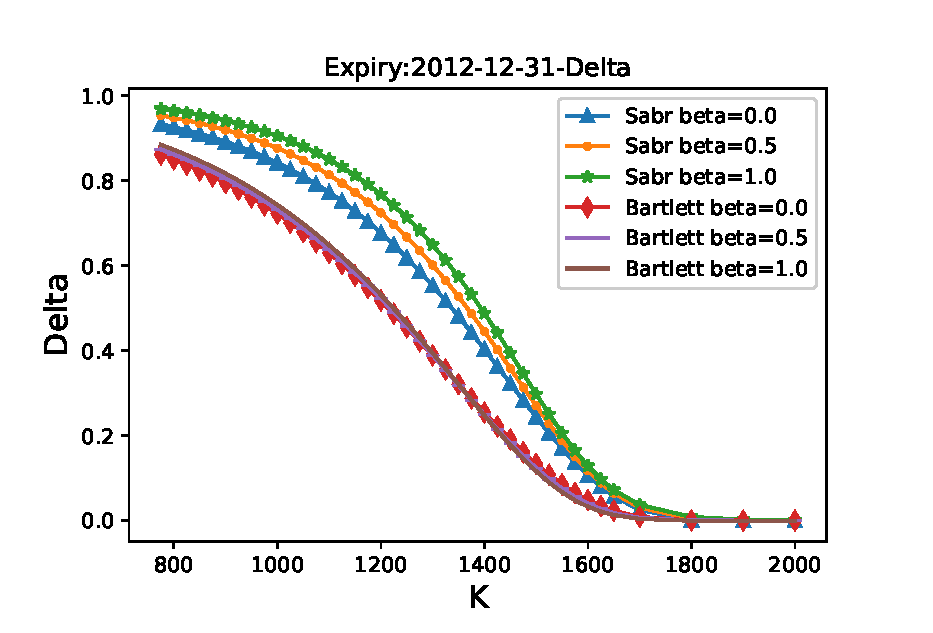
\includegraphics[width=\textwidth]{Bartlett}
	\caption{Comparison based on 2012-01-04 SP500 index option}
\end{figure}
\end{frame}


\begin{frame}{Connection with Our Research}
\begin{itemize}
	\item The dependence exists generally for all parametric pricing models.
	\item Accounting for the dependence is not always straightforward as it is under SABR models.
	\item This motivates us to directly learn a hedging position from the market data bypassing the calibration process.
\end{itemize}

\end{frame}




\section{Discussion}
\begin{frame}{Discussion}
\begin{itemize}
	\item In this talk, we discuss an efficient way of creating arbitrage-free surface and we use the surface to augment option data.
	\item We also discuss the how to adjust the delta hedging position using SABR model.
\end{itemize}
\end{frame}
\end{document}

